
\section{Mars Coordinate Frames} \label{sec:Mars} 
The generic inertial system for Mars is that defined by the IAU for solar system bodies, namely the ICRF centered on Mars \ref{sec:gen}.
The fixed frame for mars should be the one associated with its fitted gravitational field, see \ref{sec:Marsg}. As of this writing, the Mars gravity model will be MRO110B \cite{2011Icar}. For this document the fixed frame will be that defined by the IAU \ref{sec:gen}.\

\textbf{Coordinate Frame: } Rotating 

\begin{itemize}
\item X-axis: Points in the direction of the prime meridian of Mars.
\item Y-axis: Completes a standard, right-handed coordinate frame.
\item Z-axis: Defined as the pole vector of the Mars Mean Equator.
\end{itemize}

\begin{figure}[htp]
\centering
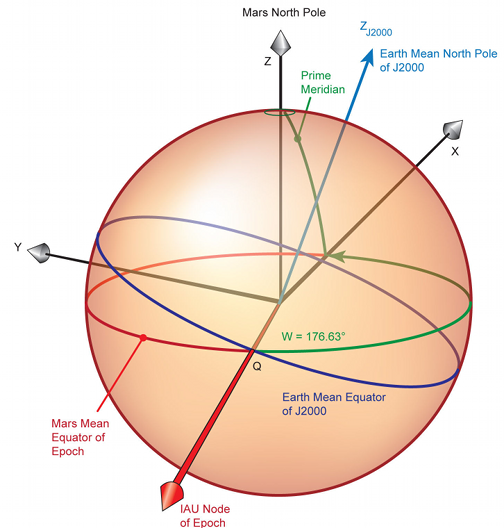
\includegraphics [width=7in]{figs/fig7.png}
\caption{Mars IAU Fixed System}
\label{fig:7}
\end{figure}

\subsection{Example MARS RNP}
See the JEOD \hypermodelref{RNP} for examples.